\chapter{Preliminarii}

\section{Tehnologii folosite}
\hspace{1cm} Aplicația WEB reprezintă un program de tip software stocat pe un server remote, devenind accesibil pentru o masă mare de utilizatori care doresc sa acceseze date rapid și ușor. Componentele sale pot  comunica prin protocoale bazate pe internet cum ar fi HTTP (Hyper Text Transfer Protocol) sau HTTPS (Hyper Text Transfer Protocol Secure).\cite{citation1}  Principalele avantaje ale aplicațiilor WEB le reprezintă accesibilitatea – acessarea lor se face folosind doar un browser WEB indiferent de circumstanțele externe (ora și loc) –, ușurința utilizatorului de a naviga pe platformă fără a avea nevoie de resurse suplimentare și scalabilitatea – poate gestiona un volum mare de date fără a se degrada –.

Aceasta are la bază arhitectura de tipul „client-server” în care clienții efectuează diferite operațiuni asupra serverului, iar răspunsurile serverului sunt primite prin intermediul internetului. 

\begin{figure}[!htb]
    \centering
    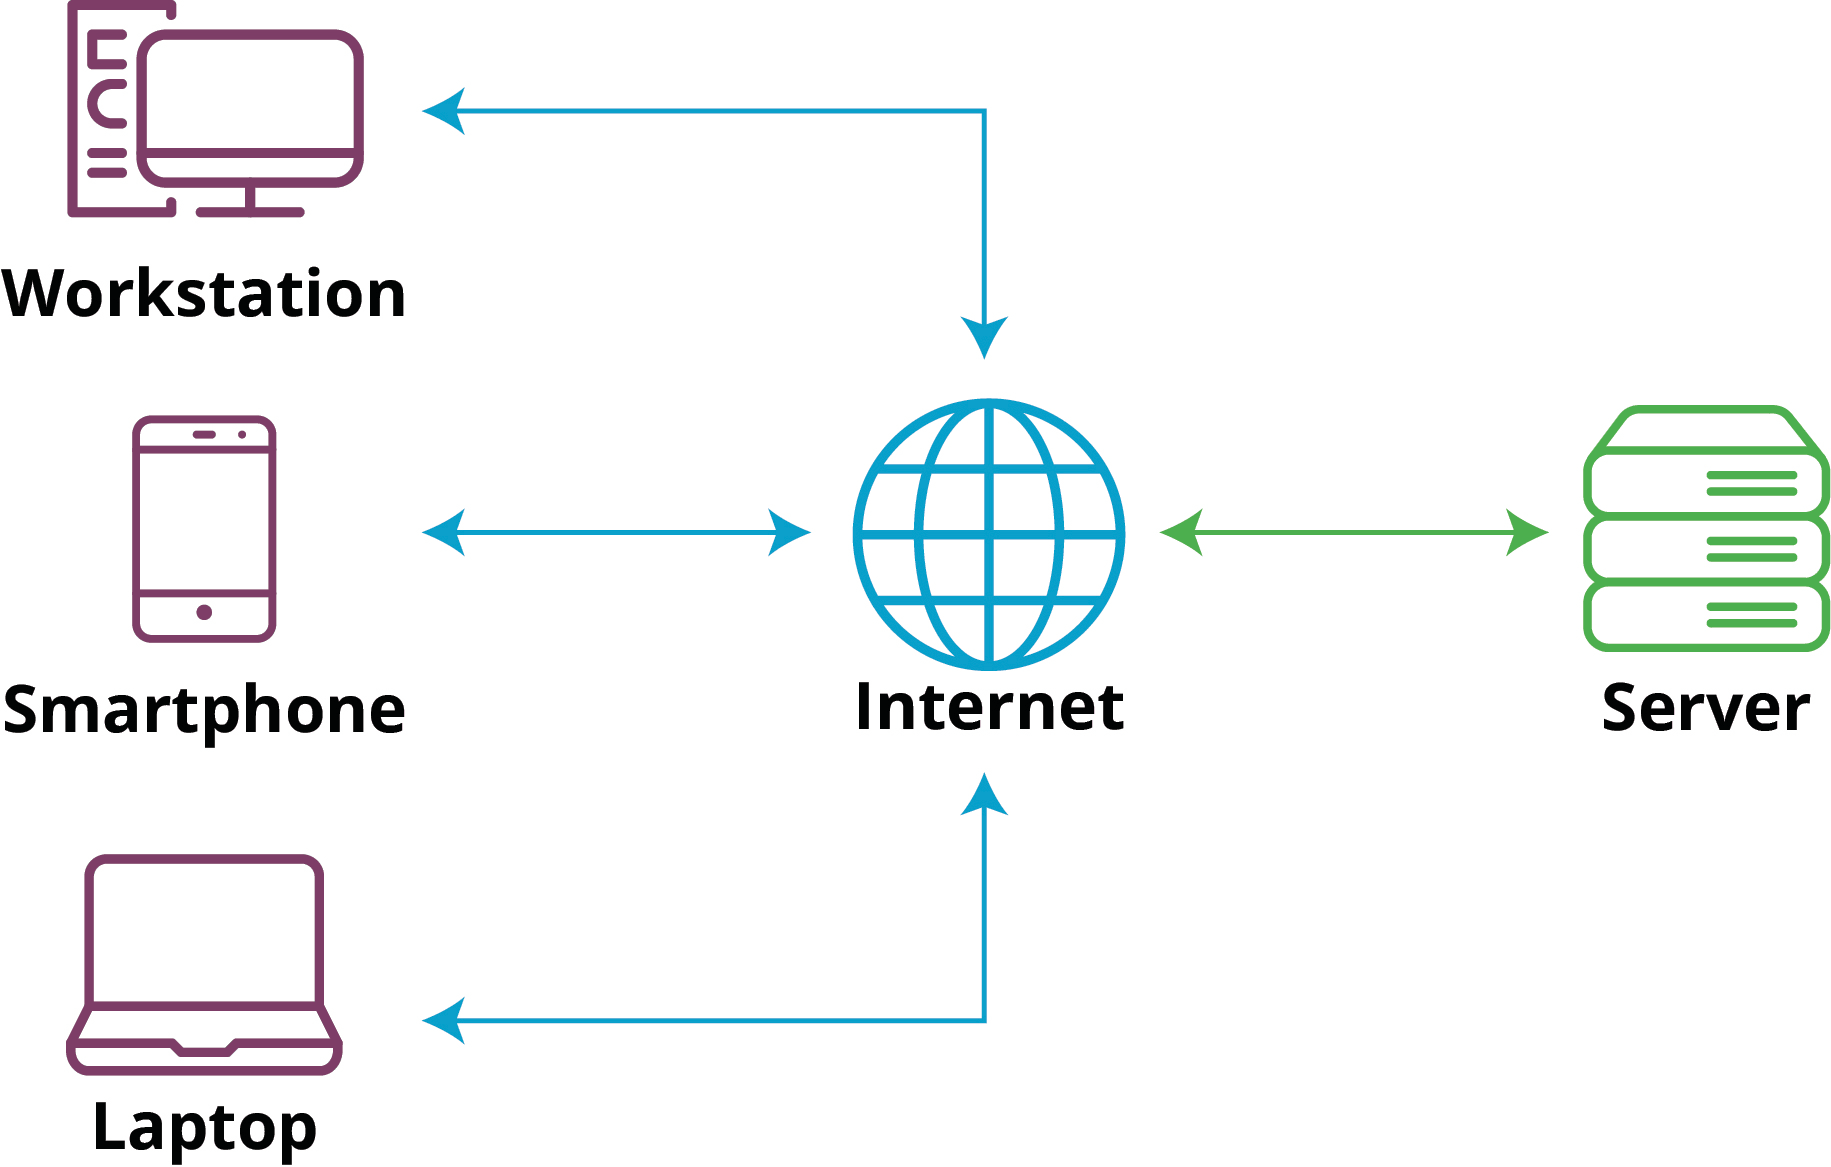
\includegraphics[width=0.7\linewidth]{images/client-server-network.png}
    \caption{Comunicarea client-server}
    \label{fig:client-server}
\end{figure}

Aplicația OfOps a fost construită având partea de server construită cu ajutorul MySQL, Spring Boot și Java, iar partea de client a fost implementată folosind instrumnete specifice frontend-ului anume Angular, HTML (HyperText Markup Language), CSS (Cascading Style Sheets) și Typescript. Aceste tehnologii vor fi descrise în subcapitolele ce urmează. 

\subsection{Stocarea datelor}
\hspace{1cm}MySQL este un sistem pentru management-ul bazelor de date relaționale, adică baze de date care stochează date în tabele separate.\cite{citation2} Structura sa este menită să fie un instrument flexibil pentru programare, întrucât poți să-ți setezi regulile după care să fie construită baza de date, relațiile între tabele (one-one, many-one, one-many, many-many), cheile primare sau străine, constrângeri etc. Utilizarea MySQL pentru stocarea bazei de date este una eficientă, întrucât modul în care această aplicație a fost construită nu permite inconsistența, duplicarea sau lipsa datelor.

Luând în considerare avantajele MySQL, am ales ca baza de date a aplicației OfOps să fie păstrată în MySQL Workbench versiunea 8.0 CE datorită volumul mare de date pe care îl suportă. Aceasta oferă o interfață intuitivă și ușor de utilizat, stocarea tabelelor este bine organizată și ai la dispoziție, printr-un singur click, detalii despre tabele, cât și datele păstrate în ele, făcând interacțiunea cu MySQL Workbench una facilă și rapidă.


\begin{figure}[!htb]
    \centering
    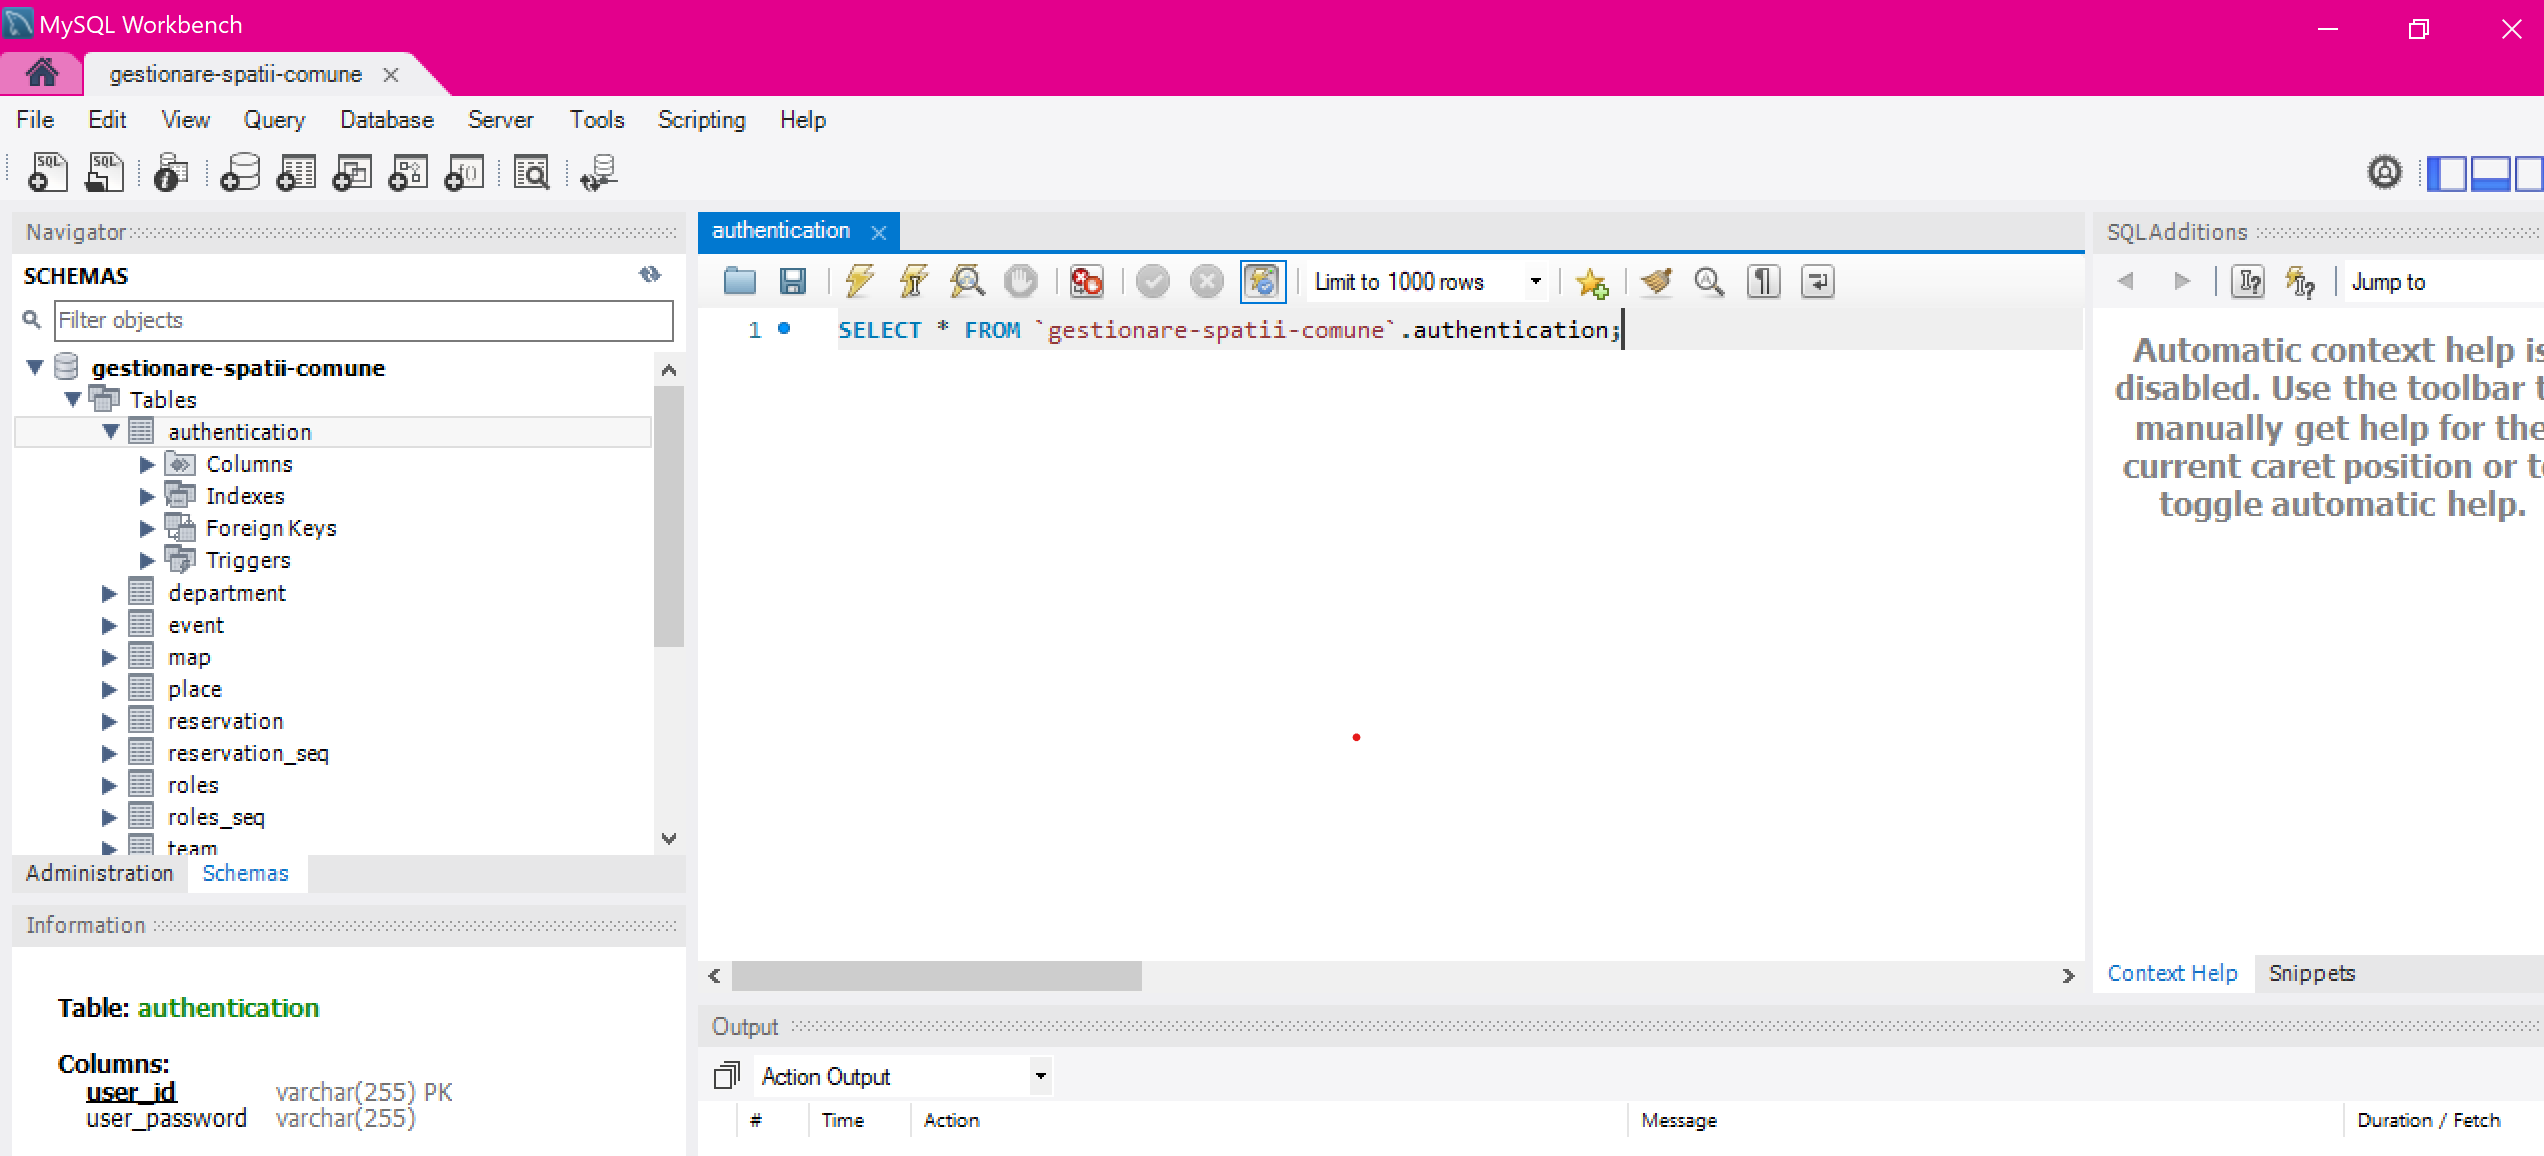
\includegraphics[width=0.9\linewidth]{images/interfata-mysql.png}
    \caption{Interfață MySQL Workbench}
    \label{fig:interfata-mysql}
\end{figure}


\subsection{Backend}
\hspace{1cm} Pentru implementarea backend-ului am utilizat Java și Spring Boot. 

\newpage

\begin{minipage}{\textwidth}
\hfill
\begin{minipage}{0.9\textwidth}
\subsubsection{Java}
\end{minipage}
\end{minipage}

\hspace{0cm} Java este un limbaj de programare orientat pe obiecte, high-level, creat in jurul anilor 1990. Până atunci, C și C++ erau cele mai răspândite limbaje de programare, însă utilizarea lor în masă largă era destul de restrânsă și costisitoare. Motivația dezvoltării Java a reprezentat-o nevoia unui limbaj de programare care să poată fi folosit pentru diferite dispozitive electronice cum ar fi cuptorul cu microunde sau chiar dispozitivele cu control remote.\cite{citation3} Versatilitatea și simplitatea acestui limbaj l-au adus printre cele mai populare și răspândite modalități de a coda până în prezent. 

De asemenea, Java joacă un rol important și în această licență, întrucât majoritatea codului dezvoltat are la bază acest limbaj de programare. Codul a necesitat instalarea în prealabil a unui JRE (Java Runtime Environment), astfel încât compilarea sa să se realizeze cu succes.

\begin{figure}[!htb]
    \centering
    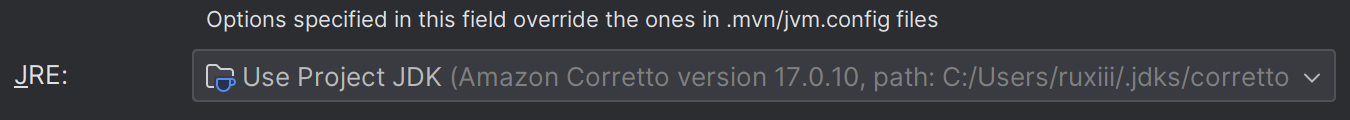
\includegraphics[width=0.9\linewidth]{images/JRE.png}
    \caption{JRE utilizat}
    \label{fig:JRE}
\end{figure}

\vspace{0.5em}
    
\begin{minipage}{\textwidth}
\hfill
\begin{minipage}{0.9\textwidth}
\subsubsection{Spring Boot}
\end{minipage}
\end{minipage}

\hspace{0cm}Spring este un framework care vine în ajutorul dezvoltării rapide ale unor aplicații stand-alone, deoarece lucrează cu alte librării astfel încât construirea aplicației să nu mai aibă nevoie de de o configurare foarte mare în plus.\cite{citation4}

Am ales Maven pentru adăugarea dependințelor, iar pe lângă cele deja integrate în proiect am mai adăugat: Spring-Boot-Starter-Data-JPA (interacțiune backend - baza de date), Spring-Boot-Starter-WEB (simplifică construirea aplicațiilor WEB cu Spring), MySQL-Connector-J (conexiunea cu baza de date), Lombok (generare de cod comun), Spring-Boot-Starter-Test (pentru testele unitare), Spring-Boot-Starter-Security și Java-JWT (pentru securitatea aplicației).

\vspace{1.5em}
\subsection{Frontend}
\hspace{1cm} Pentru implementarea frontend-ului am utilizat Angular, HTML, CSS și TypeScript.

\begin{minipage}{\textwidth}
\hfill
\begin{minipage}{0.9\textwidth}
\subsubsection{Angular}
\end{minipage}
\end{minipage}

\hspace{0cm} Angular este un framework pentru frontend care ajută la crearea unei aplicații de tipul single-page. Ce diferențiază Angular de celelalte framework-uri pentru frontend este strucutura sa bazată pe componente. Astfel, scheletul codului este mai ușor de organizat, deoarece fiecare componentă are rolul ei bine definit, iar identificarea unei potențiale greșeli este mai ușor de găsit.\cite{citation5}

\newpage

\begin{center}
\begin{minipage}{0.8\textwidth}
\captionsetup{type=listing}
   \begin{lstlisting}
@Component({
  selector: 'app-my-reservation',
  templateUrl: './my-reservation.component.html',
  styleUrl: './my-reservation.component.css'
})
export class MyReservationComponent { }
\end{lstlisting} 
\end{minipage}
\end{center}


\vspace{0.5em}


\begin{minipage}{\textwidth}
\hfill
\begin{minipage}{0.9\textwidth}
\subsubsection{HTML}
\end{minipage}
\end{minipage}

\hspace{0cm} Expunerea componentelor din Angular se realizează în pagină cu ajutorul elementelor de HTML. Acesta oferă o structurare bine pusă la punct conținutului paginii, existând diferențe între tipuri de text (titlu, bold, itallic etc.), liste, tabele și multe altele elemente care fac experiența user-ului în aplicație cât mai placută. 

\begin{center}
\begin{minipage}{0.8\textwidth}
\captionsetup{type=listing}
   \begin{lstlisting}
 <h1>Account created successfully!
        <br/> Don't forget your user ID for login!</h1>
\end{lstlisting} 
\end{minipage}
\end{center}

\vspace{0.5em}

\begin{minipage}{\textwidth}
\hfill
\begin{minipage}{0.9\textwidth}
\subsubsection{CSS}
\end{minipage}
\end{minipage}

\hspace{0cm} Înfrumusețarea aplicației și, implicit, a tag-urilor HTML se efectuează cu ajutorul modurilor de stilizare din CSS. Ele au scopul să creeze un aspect vizual inedit al aplicației, raportândune-ne de la culorile de background ale aplicației până la mici elemente de finețe cum ar fi alerte sau butoane.

\begin{center}
\begin{minipage}{0.8\textwidth}
\captionsetup{type=listing}
   \begin{lstlisting}
h1{
    text-align: center;
    font-size: 40px;
    font-weight: bold;
}
\end{lstlisting} 
\end{minipage}
\end{center}

\vspace{0.5em}

\begin{minipage}{\textwidth}
\hfill
\begin{minipage}{0.9\textwidth}
\subsubsection{TypeScript}
\end{minipage}
\end{minipage}

\hspace{0cm} Typescript este cel mai important limbaj pentru dezvoltarea unei aplicații în Angular. Multitudinea avantajelor acestuia precum folosirea interfețelor și claselor, structura simplă și ușor de înțeles, îmbinarea caracteristicilor de JavaScript cu declararea statică a tipurilor de date fac TypeScript-ul temelia unei aplicații în Angular.

\begin{center}
\begin{minipage}{0.8\textwidth}
\captionsetup{type=listing}
   \begin{lstlisting}
export class DepartmentsComponent {
  departmentId: string;
  departmentName: string;
}
\end{lstlisting} 
\end{minipage}
\end{center}

\vspace{1.5em}
\section{Asigurarea securității}

\section{Mijloace de testare}

